\documentclass[letterpaper, 10 pt, conference]{ieeeconf}
%\documentclass[a4paper, 10pt, conference]{ieeeconf}

\IEEEoverridecommandlockouts
\overrideIEEEmargins

% The following packages can be found on http:\\www.ctan.org
\usepackage{graphicx} % for pdf, bitmapped graphics files
%\usepackage{epsfig} % for postscript graphics files
%\usepackage{mathptmx} % assumes new font selection scheme installed
%\usepackage{times} % assumes new font selection scheme installed
\usepackage{amsmath} % assumes amsmath package installed
\usepackage{amssymb}  % assumes amsmath package installed

\usepackage{url}
\usepackage{ae} % Nice Slovak symbols
\usepackage{listings,lstautogobble} % Nice MATLAB source code
\usepackage{matlab-prettifier}

\title{\LARGE \bf
A software package for MPC design and tuning: MPT+
}

\author{Juraj Holaza, Lenka Gal\v{c}\'{i}kov\'{a}, Juraj Oravec, Michal Kvasnica
\thanks{Authors are with Faculty of Chemical and Food Technology,
		Slovak University of Technology in Bratislava, Bratislava, SK-812 37, Slovakia
        \texttt{lenka.galcikova@stuba.sk}}
}

\begin{document}



\maketitle
\thispagestyle{empty}
\pagestyle{empty}

\begin{abstract}

[ TOOD: Think of the better title. ]

[ TOOD: Write an Abstract ]

\end{abstract}

\section{Introduction}
\label{sec:introduction}

[ TOOD: Write an Introduction ]

% MOVED
The MPC design problem is addressed in plenty of well-developed software tools. Most of the packages provide dedicated built-in solvers, and the other delegate the optimization problem to third-party solvers. 

Following is a brief review of the MPC design software limited just for the tools offering an interface for the \texttt{MATLAB}\footnote{\texttt{MATLAB}, MathWorks, Inc.: \texttt{\url{https://www.mathworks.com}}} programming environment. We refer the reader to~\cite{KF18,LT17,HS22}, 
% ~\cite{KF18,LT17, OSQP,QPALM,qpDUNES,Ferreau2014,HPIPM,CVXGEN,EJ21,HS22}, 
and the references therein, for the review on the tailored solvers and tools supporting MPC design and its evaluation using also other programming environments, e.g., \texttt{Python}\footnote{\texttt{Python}, Python Software Foundation: \texttt{\url{https://www.python.org}}}, \texttt{Julia} \footnote{\texttt{Julia}, JuliaLang.org: \texttt{\url{https://julialang.org}}}, etc. Such the packages include QP-solvers \texttt{qpDUNES}~\cite{qpDUNES}, \texttt{QPALM}~\cite{QPALM}, \texttt{CVXGEN}~\cite{CVXGEN}, and the tools introducing the distributed optimization \texttt{OSQP}~\cite{OSQP}, \texttt{ALADIN}-$\alpha$~\cite{EJ21}, to name a few. 
% \texttt{Python}~\cite{PYTHON}, \texttt{Julia}~\cite{JULIA}, etc.

Commercial \texttt{MPC Toolbox}~\cite{MPC_toolbox} for \texttt{MATLAB} addresses various classes of the MPC design problems, including the construction of the adaptive, explicit, gain-scheduled, and non-linear MPC controllers. This toolbox provides several built-in solvers and also a dedicated user interface \texttt{MPC Designer App} for the controller tuning. 
%
The non-linear MPC design problems are efficiently solved using the \texttt{ACADO Toolkit}~\cite{ACADO_Toolkit}. The non-convex optimization problem is solved by the sequential quadratic programming (SQP) approach.  \texttt{ACADO Toolkit} evaluates the library-dependent \texttt{C/C++} code and provides an interface for \texttt{MATLAB}. 
%
\texttt{CasADi}~\cite{CasADi} represents another toolbox suitable for the non-liner MPC design. This open-source package also provides the interfaces for \texttt{MATLAB} and \texttt{Python}. 
%
The non-linear MPC can be designed also using the open-source toolbox \texttt{MATMPC}~\cite{MATMPC}. 
%
\texttt{YALMIP}~\cite{L04} toolbox is a widely-used modelling parser focused on the various classes of optimization problems, including non-convex optimization. \texttt{YALMIP} provides also support for the MPC design problems. 
%
Similar to \texttt{YALMIP} toolbox, the \texttt{CVX}~\cite{GB08} is focused on the modelling of the various classes of convex optimization problems suitable for MPC controller design. 

[ TODO: Introduce MPT ]

\texttt{MPT} module \texttt{LowCom}~\cite{KH15} introduces the set of methods reducing the complexity of the explicit solution maps associated with the MPC controllers.

[ TODO: Introduce Tube MPC ]

Moreover, Tube MPC represents a natural step towards the stochastic and non-linear MPC design. Finally, due to the ability to handle the quantized control variables, Tube MPC is also a necessary tool in a highly relevant field of the encrypted MPC design using the cloud-computing services, e.g., see~\cite{DR18} and the related works.

[ TODO: Reformulate: ]

We present the new package \texttt{MPTplus} extending the original \texttt{MPT} toolbox by the ability to design, tune, and validate both, non-explicit (implicit) and explicit Tube MPC controllers in a memory-efficient and user-friendly way.
Next, we provide an extensive case study investigating the benefits of the developed package considering the advanced robust control of the laboratory device Flexy~\cite{CK19}. 

\section{Theoretical backgrounds}
\label{sec:tube_mpc_theory}

[ TOOD: Write the theoretical backgrounds on Tube MPC. ]

[ TODO: Reformulate ]

This section briefly reviews the main theoretical backgrounds of the original (rigid) Tube MPC design approach proposed in~\cite{MS05} and its formulation considering multi-parametric optimization.

\subsection{Tube MPC design}
\label{sec:tube_mpc}

Consider an uncertain linear time-invariant (ULTI) system in the form:
\begin{eqnarray}
	\label{eq:ulti_system}
	x(t+T_{\mathrm{s}}) = A x(t) + B u(t) + E d(t), % \quad x(0) = x_{0},
\end{eqnarray}
where $t$ stands for the time instant in the discrete-time domain determined by the given sampling time $T_{\mathrm{s}}$. $A \in \mathbb{R}^{n_{\mathrm{n}_{x}} \times n_{\mathrm{n}_{x}}}$ is system matrix, $B \in \mathbb{R}^{n_{\mathrm{n}_{x}} \times n_{\mathrm{n}_{u}}}$ is input matrix, such that the matrix pair $(A,B)$ is stabilizable. $E \in \mathbb{R}^{n_{\mathrm{n}_{x}} \times n_{\mathrm{n}_{w}}}$ is disturbance matrix, $x \in \mathbb{R}^{n_{\mathrm{x}}}$ is the vector of the system states, $u \in \mathbb{R}^{n_{\mathrm{u}}}$ is control action, $d \in \mathbb{D} \subset \mathbb{R}^{n_{\mathrm{x}}}$ is bounded additive disturbance such that $\mathbb{D}$ is compact set containing the origin. 

For the sake of notation, in ULTI system~\eqref{eq:ulti_system} holds:
\begin{eqnarray}
	\label{eq:disturbance_set}
	w = E \, d, ~ w \in \mathbb{W}, ~ \mathbb{W} = \left\{ w \in \mathbb{R}^{n_{\mathrm{x}}} : \Vert w \Vert_{\infty} \leq w_{\max} \right\}
\end{eqnarray}
for given upper bound value $w_{\max} = \Vert E \, d \Vert_{\infty}$, $\forall d \in \mathbb{D}$ such that $\mathbb{W} \supseteq E \, \mathbb{D}$ is the minimum volume hyper-box satisfying $\Vert w \Vert_{\infty} = w_{\max}$.

Moreover, the ULTI system in~\eqref{eq:ulti_system} is subject to state and input constraints
\begin{eqnarray}
	\label{eq:constraints_x_u}
	x(t) \in \mathbb{X}, \quad u(t) \in \mathbb{U}, \quad \forall t \geq 0,
\end{eqnarray}
where $\mathbb{X} \in \mathbb{R}^{n_{\mathrm{x}}}$ and $\mathbb{U} \in \mathbb{R}^{n_{\mathrm{u}}}$ are polytopes, i.e., compact sets, containing origin in their strict interiors. 

The ``tube'' introduced into the MPC design is evaluated by the convex set $\mathbb{T} \subset \mathbb{R}^{n_{\mathrm{x}}}$ and represents the origin for the perturbed system, see~\cite{MS05}. 
%
By plugging the LQ-optimal controller into~\eqref{eq:ulti_system} and updating the additive disturbances per~\eqref{eq:disturbance_set}, we obtain an autonomous discrete-time uncertain system 
\begin{equation}
	\label{eq:autosys}
	x(t+T_{\mathrm{s}}) = (A + BK)x(t) + w(t).
\end{equation}
Subsequently, if $\mathbb{T}$ is a robust positive invariant (RPI) set for~\eqref{eq:autosys}, then we have that following statement holds 
\begin{eqnarray}
	\label{eq:tube}
	\left( A + B K \right) \mathbb{T} \oplus \mathbb{W} \subseteq \mathbb{T},
\end{eqnarray}
where $\oplus$ denotes the Minkowski sum.

Obviously, $\mathbb{T}$ in \eqref{eq:tube} is constructed as the minimal RPI set to minimize the conservativeness of Tube MPC design by:
\begin{eqnarray}
	\label{eq:tube_design}
	\mathbb{T} = \sum_{i=0}^{\infty} \left( A + B K \right)^{i} \mathbb{W},
\end{eqnarray}
where $\Sigma$ represents a set addition. However, if the $K$ is not a dead-beat controller, then the minimal RPI set $\mathbb{T}$ does not necessarily lead to the polytope, see~\cite{MS05}. Therefore, $\mathbb{T}$ is designed as the outer approximation of the minimal RPI set.  Algorithm constructing such invariant approximations of the minimal robust positively invariant set $\mathbb{T}$ is proposed in detail in~\cite{RK05}.

The conventional (rigid) Tube MPC design problem has the form:
\begin{subequations}
	\label{eq:tmpc}
	\begin{eqnarray}
		\label{eq:tmpc_cost}
		\min_{\hat{u}_{0},\ldots,\hat{u}_{N-1}, \hat{x}_{0},\ldots,\hat{x}_{N} } \!\!\!\!\!\!\!\!\!\!\! &\,& \Vert \hat{x}_{N} \Vert_{P}^{2} + \sum_{k=0}^{N-1} \left( \Vert \hat{x}_{k} \Vert_{Q}^{2} + \Vert \hat{u}_{k} \Vert_{R}^{2} \right) \qquad \\
		\label{eq:tmpc_rpi}
		\mathrm{s.t.\!:} &\,& x(t) - \hat{x}_{0} \in \mathbb{T} , \\
		\label{eq:tmpc_model}
		&\,&  \hat{x}_{k+1} = A \hat{x}_{k} + B \hat{u}_{k} , \\
		\label{eq:tmpc_constraints_state}
		&\,& \hat{x}_{k} \in \mathbb{X} \ominus \mathbb{T} , \\
		\label{eq:tmpc_constraints_terminal}
		&\,& \hat{x}_{N} \in \mathbb{X}_{\mathrm{N}}, \\
		\label{eq:tmpc_constraints_input}
		&\,& \hat{u}_{k} \in \mathbb{U} \ominus K \, \mathbb{T} , \\
		\label{eq:tmpc_constraints_input_delta_k}
		&\,& \Delta \hat{u}_{l} \in \mathbb{U}_{\Delta} \ominus K \, \mathbb{T} , \\
		\label{eq:tmpc_constraints_input_delta_0}
		&\,& \hat{u}_{k} + K ( x(t) - \hat{x}_{0} ) - u(t_{-}) \in \mathbb{U}_{\Delta} , \quad
	\end{eqnarray}
\end{subequations}
where $\forall k = 0, \dots, N-1$,  $\forall l = 1, \dots, N-1$, $N$ is prediction horizon.
The decision variables\footnote{Obviously, dense formulation of~\eqref{eq:tmpc} omits $\hat{x}_{k}$ as the decision variables, except for $\hat{x}_{0}$.} $\hat{u}_{k}$, $\hat{x}_{k}$, are optimized subject to the nominal system behaviour in~\eqref{eq:tmpc_model}, i.e., an idealized system without the impact of any uncertain parameters. The state and input constraints in~\eqref{eq:constraints_x_u} are respectively adopted in~\eqref{eq:tmpc_constraints_state}, \eqref{eq:tmpc_constraints_input} to respect the RPI set $\mathbb{T}$ in~\eqref{eq:tube} assuming: $(\mathbb{X} \ominus \mathbb{T})$, $(\mathbb{U} \ominus K \, \mathbb{T})$ are non-empty sets, convex by definition. Analogous, the initial condition in~\eqref{eq:tmpc_rpi} takes into account the RPI set $\mathbb{T}$ keeping the perturbed system state vector $x(t)$ close to its nominal counterpart $\hat{x}_{0}$. 
The terminal constraint in~\eqref{eq:tmpc_constraints_terminal} has the conventional form.
The quadratic cost function in~\eqref{eq:tmpc_cost} is minimized considering the $Q$, $R$, $P$. Note, $\Vert \hat{x}_{N} \Vert_{P}^{2}$ denotes simplified notation for the weighted two norm: $\hat{x}_{N}^{\top} P \hat{x}_{N}$, and analogous hold for the remaining terms. 
The corresponding stability and recursive feasibility proofs of~\eqref{eq:tmpc} are documented in~\cite{MS05}.

The control action $u(t)$, which is applied to the controlled plant in~\eqref{eq:ulti_system}, is determined by the control law $\kappa : \mathbb{X}_{\mathrm{F}} \rightarrow \mathbb{U}$
\begin{eqnarray}
	\label{eq:tmpc_control_law}
	\kappa(x(t)) = \hat{u}_{0}^{\star} + K \left( x(t) - \hat{x}_{0}^{\star} \right),
\end{eqnarray}
where $\star$ denotes the solution of the optimization problem in~\eqref{eq:tmpc} and $\mathbb{X}_{\mathrm{F}} \subseteq \mathbb{R}^{n_{\mathrm{x}}}$ is the corresponding domain, i.e., the feasibility set of the optimized initial conditions $\hat{x}_{0}$ of~\eqref{eq:tmpc}. 
Tube MPC is implemented in receding horizon fashion, i.e., just the first control action $u(t) = \kappa(x(t))$ is applied to the plant and the optimization problem in~\eqref{eq:tmpc} is re-computed in each control step. 

%% OUTPUT TUBE MPC
%
%The output feedback Tube MPC design problem has the form:
%\begin{subequations}
%	\label{eq:tmpc_output}
%	\begin{eqnarray}
%		\label{eq:tmpc_output_cost}
%		\min_{\hat{u}_{0},\ldots,\hat{u}_{N-1}, \hat{x}_{0},\ldots,\hat{x}_{N} } \!\!\!\!\!\!\!\!\!\!\! &\,& \Vert \hat{x}_{N} \Vert_{P}^{2} + \sum_{k=0}^{N-1} \left( \Vert \hat{x}_{k} \Vert_{Q}^{2} + \Vert \hat{u}_{k} \Vert_{R}^{2} \right) \qquad \\
%		\label{eq:tmpc_output_rpi}
%		\mathrm{s.t.\!:} &\,& x(t) - \hat{x}_{0} \in \mathbb{T}_{\mathrm{x}} , \\
%		\label{eq:tmpc_output_model}
%		&\,&  \hat{x}_{k+1} = A \hat{x}_{k} + B \hat{u}_{k} , \\
%		\label{eq:tmpc_output_constraints_state}
%		&\,& \hat{x}_{k} \in \mathbb{X} \ominus \mathbb{T} , \\
%		\label{eq:tmpc_output_constraints_terminal}
%		&\,& \hat{x}_{N} \in \mathbb{X}_{\mathrm{N}}, \\
%		\label{eq:tmpc_output_constraints_input}
%		&\,& \hat{u}_{k} \in \mathbb{U} \ominus K \, \mathbb{T}_{\mathrm{x}} , \\
%		% \label{eq:tmpc_output_constraints_input_delta_k}
%		% &\,& \Delta \hat{u}_{l} \in \mathbb{U}_{\Delta} \ominus K \, \mathbb{T} , \\
%		\label{eq:tmpc_output_constraints_input_delta_0}
%		&\,& \hat{u}_{k} + K ( x(t) - \hat{x}_{0} ) - u(t_{-}) \in \mathbb{U}_{\Delta} , \quad
%	\end{eqnarray}
%\end{subequations}
%where $\forall k = 0, \dots, N-1$,  $\forall l = 1, \dots, N-1$, $N$ is prediction horizon.
%
%$\mathbb{T} = \mathbb{T}_{\mathrm{y}} \oplus \mathbb{T}_{\mathrm{x}}$

\subsection{Explicit Tube MPC}
\label{sec:explicit_mpc}

% [ TODO: Write about explicit Tube MPC. ]
The main benefit of explicit MPC is its ability to significantly speed up the real-time evaluation of the optimal control action by pre-computing the optimization problem in advance, see~\cite{BM02}. Simultaneously, the explicit solution provides the possibility for rigorous analysis, verification, and certification of the designed control law. 

The QP in~\eqref{eq:tmpc} can be reformulated into the explicit MPC design framework by evaluating the initial condition in~\eqref{eq:tmpc_rpi} exploring the set of admissible initial conditions: $\Theta = \mathbb{X} \ominus \mathbb{T}$. Then, the solution of corresponding multi-parametric QP (mpQP) returns also the convex set of feasible system states $\mathbb{X}_{\mathrm{F}} \subseteq \Theta$ defined as the explicit solution map:
\begin{eqnarray}
	\label{eq:tmpc_partition}
	\mathbb{X}_{\mathrm{F}} = \bigcup_{i}^{n_{\mathrm{r}}} \mathcal{P}_{i} ,
\end{eqnarray}
where $\mathcal{P}_{i}$ are polytopes, i.e., critical regions, and $n_{\mathrm{r}}$ is the total number of critical regions.

As the consequence, for $x(t) \in \mathcal{P}_{i}$ denoting $i$th critical region, holds control law in~\eqref{eq:tmpc_control_law} given in a form of
piece-wise affine (PWA) functions corresponding to the particular decision variables:
\begin{subequations}
	\label{eq:tmpc_control_law_pwa_particular}
	\begin{eqnarray}
		\label{eq:tmpc_control_law_pwa_particular_x}
		\hat{x}^{\star}(x(t)) \!\!\!\!&=&\!\!\!\! F_{\mathrm{x},i} \, x(t) + g_{\mathrm{x},i} \quad \text{if} \quad x(t) \in \mathcal{P}_{i}, \\
		\label{eq:tmpc_control_law_pwa_particular_u}
		\hat{u}^{\star}(x(t)) \!\!\!\!&=&\!\!\!\! F_{\mathrm{u},i} \, x(t) + g_{\mathrm{u},i} \quad \text{if} \quad x(t) \in \mathcal{P}_{i},
	\end{eqnarray}
\end{subequations}
where $F_{\mathrm{x},i}$, $F_{\mathrm{u},i}$, $g_{\mathrm{x},i}$, $g_{\mathrm{u},i}$ have appropriate dimensions. For further technical details see~\cite{BM02}. 
Analogous to~\cite{ZT14}, we re-formulate the control law of the explicit Tube MPC in~\eqref{eq:tmpc_control_law_pwa_particular} into the compact form:
\begin{eqnarray}
	\label{eq:tmpc_control_law_pwa}
	\kappa(x(k)) = \underbrace{ \left( K + F_{\mathrm{x},i} + F_{\mathrm{u},i} \right) }_{ F_{i} } x(k) + \underbrace{ \left( g_{\mathrm{u},i} - K g_{\mathrm{x},i} \right) }_{ g_{i} } ,
\end{eqnarray}
We point out, that such a compact formulation significantly reduces the associated memory footprint necessary to store the PWAs compared to the conventional explicit formulation in~\eqref{eq:tmpc_control_law_pwa_particular}.  
%
To be specific, the feedback law in~\eqref{eq:tmpc_control_law_pwa} saves $3\,n_\text{x}$ double precision numbers per each critical region compared to the original form~\eqref{eq:tmpc_control_law_pwa_particular_x}.
%
%	The memory savings related to storage of the set of $n_{\mathrm{r}}$ matrix pairs $(F_{\mathrm{x},i}, F_{\mathrm{u},i})$ compared to $F_{i}$ is, roughly, decreased by factor 2, and further savings related to pairs of vectors $(g_{\mathrm{x},i}, g_{\mathrm{u},i})$ compared to $g_{i}$ corresponds to $( n_{\mathrm{r}} \times n_{\mathrm{x}} )$ double-precision numbers.

\section{The software package}
\label{sec:code}

[ TOOD: Describe a software package. ]

\subsection{MPT+}
\label{sec:code_mptplus}

[ TOOD: Describe an MPT+ package. ]

The \texttt{MPTplus} toolbox extends the functionality of the \texttt{MPT} toolbox~\cite{MPT3}. In this section, we introduce the novel features, including (i) efficient explicit Tube MPC controller construction, (ii) introducing incremental constraints into the Tube MPC design, and (iii) the general polynomial approximation of the PWA control law. 

\subsection{Installation}
\label{sec:installation}

The \texttt{MPTplus} toolbox is freely available at \texttt{GitHub}\footnote{\texttt{MPTplus: \url{https://github.com/holaza/mptplus}}}. We recommend to install the package via \texttt{tbxManager}\footnote{\texttt{tbxManager: \url{https://www.tbxmanager.com}}} by typping:
\begin{lstlisting}[style=Matlab-editor]
	tbxmanager install mptplus
\end{lstlisting}
Alternatively, install the \texttt{MPTplus} by setting the corresponding path in \texttt{MATLAB}. 

\subsection{Advanced methods for explicit Tube MPC controllers}
\label{sec:advanced_method}

% [ TODO: Write about the advanced methods of the MPT toolbox available for Tube MPC. ]
This section lists the current compatibility\footnote{The package \texttt{MPTplus} is still under development and further extensions are expected, soon.} of \texttt{MPTplus} with \texttt{MPT}. 
%
Since the implicit MPC policy \verb|TMPC| is currently restricted only to evaluation via \verb|TMPC.optimizer(x)|, for any feasible state vector $x\in\mathbb{X}_{\mathrm{F}}$, we devote this section to its explicit counterpart \verb|ETMPC|.

Assume that from the previous Section~\ref{sec:construction} we have defined \verb|model|, i.e., object that contains prediction model~\eqref{eq:example_ulti_system} as in~\eqref{eq:tmpc_model}, constraints~\eqref{eq:constraints_x_u} transformed into~\eqref{eq:tmpc_constraints_state}-\eqref{eq:tmpc_constraints_input}, penalty matrices, the appertain LQR terminal penalty and terminal set as in~\eqref{eq:tmpc_cost} and~\eqref{eq:tmpc_constraints_terminal}, respectively. 
%
Using the \texttt{MPTplus}, we may simply construct both, non-explicit and explicit Tube MPC controllers\footnote{The current version of \texttt{MPTplus} always displays for explicit Tube MPC controller confusing information on the prediction horizon $N=1$, although the controller is constructed correctly for any value of $N$.}. To design explicit MPC policy that returns the control action as in~\eqref{eq:tmpc_control_law}, i.e., that is fed directly to the controlled system in~\eqref{eq:ulti_system}, we can evoke:
\begin{lstlisting}[style=Matlab-editor]
ETMPC = TMPC.toExplicit
\end{lstlisting}
what constructs explicit controller \verb|ETMPC| that is defined over $n_\text{r} = 565$ critical regions in $n_\text{x} = 2$ dimensional space.

To graphically analyze our explicit controller, we can type:
\begin{lstlisting}[style=Matlab-editor]
figure; ETMPC.partition.plot()
figure; ETMPC.feedback.fplot()
figure; ETMPC.cost.fplot()
\end{lstlisting}
to plot the polytopic partition~\eqref{eq:tmpc_partition}, the PWA feedback law~\eqref{eq:tmpc_control_law_pwa}, and the PWQ value function as defined in~\eqref{eq:tmpc_cost}, respectively.\footnote{We note that while both, the PWA feedback law and the PWQ value function, are given as solution to~\eqref{eq:tmpc} the solution~\eqref{eq:tmpc_control_law_pwa_particular} was posterior transformed into~\eqref{eq:tmpc_control_law_pwa}, however, the value function preserves its form of~\eqref{eq:tmpc_cost}.}

To perform a closed-loop simulation of a computed explicit Tube MPC controller one can define an object:
\begin{lstlisting}[style=Matlab-editor]
	loop = ClosedLoop(ETMPC,model)
\end{lstlisting}
where \verb|model| can contain even a modified version of~\eqref{eq:example_ulti_system}, i.e., the controlled system can be different from the prediction model used to design the explicit policy \verb|ETMPC|. Subsequently, we can execute the closed-loop simulation by:
\begin{lstlisting}[style=Matlab-editor]
Nsim = 10
data = loop.simulate(x0, Nsim)
\end{lstlisting}	
with \verb|x0| denoting the initial condition and \verb|Nsim| number of the closed-loop simulation steps. The generated \verb|data| structure contains all important information, e.g., the closed-loop profiles of control inputs \verb|data.U|, applied disturbances \verb|data.D|, states \verb|data.X|, and the cost of~\eqref{eq:tmpc_cost} at each time step, to name a few.
Alternatively, one can create a customized loop, where the control input of \verb|ETMPC| can be obtained by typing: 
\begin{lstlisting}[style=Matlab-editor]
u = ETMPC.evaluate(x)
\end{lstlisting}
for any given feasible state vector $x\in\mathbb{X}_{\mathrm{F}}$.
%
Finally, if only pure visual analysis of a closed-loop simulation is required then we encourage users to use
\begin{lstlisting}[style=Matlab-editor]
ETMPC.clicksim()
\end{lstlisting}
where initial state conditions are defined by the mouse.
%
%	Finally, for more rigorous verification of closed-loop stability we encourage a user to create a Lyapunov function $V$ that provides $V(x(k))>0$, $V(0)=0$, $V(x(k+1)) \leq \gamma V(x(k))$ for all $x(k) \in \mathbb{X}_{\mathrm{F}}$, some $\gamma \in [0,1)$, and all $k \geq 0$. This can be done easily by 
%	\begin{lstlisting}[style=Matlab-editor]
	%		lyap = loop.toSystem.lyapunov(type)
	%	\end{lstlisting}

Another interesting group of \texttt{MPT} features is the module \texttt{LowCom}~\cite{KH15} that provides various complexity reduction techniques of explicit MPC policies. In this paper, we list techniques that do not induce suboptimality\footnote{Currently, complexity reduction schemes that introduce suboptimality are not compatible with the Tube MPC.}.

The Optimal Region Merging (ORM) method aims to join critical regions with the same closed-loop feedback policy and whose union is a convex set. This method can be called: 
\begin{lstlisting}[style=Matlab-editor]
ETMPCsim = ETMPC.simplify('orm')
\end{lstlisting}
where \verb|ETMPCsim| is the constructed simplified controller. In our setup, this technique found $158$ critical regions that were merged. Hence, we have reduced the complexity by $28\%$ as the number of critical regions dropped from $565$ to $407$. 

%
%	The clipped-based method targets to achieve complexity reduction by removing all critical regions with saturated control law. Subsequently, to cover the entire original polytopic partition $\mathbb{X}_{\mathrm{F}}$, critical regions with unsaturated control law are extended and a clipping filter is introduced. This method can be called by 
%	\begin{lstlisting}[style=Matlab-editor]
	%	simpleETMPC = ETMPC.simplify('clipping')
	%	\end{lstlisting}
%	where \verb|simpleETMPC| denotes the resulting simplified controller. With our setup, 
%
The separation-based method targets to reduce the complexity of explicit controllers by removing all critical regions that lead to the saturated control laws, i.e., $u(t)$ that lay on the boundary of $\mathbb{U}$. Once this is done, a separation filter is constructed to identify optimal control actions above the removed critical regions. This simplification method is called:
\begin{lstlisting}[style=Matlab-editor]
ETMPCsim = ETMPC.simplify('separation')
\end{lstlisting}
where \verb|ETMPCsim| denotes the resulting simplified controller. With the considered control setup, the separation-based controller has removed all $120$ regions with saturated feedback law which represents the reduction of $21\%$ w.r.t. its complex counterpart \verb|ETMPC|.

Needlessly to say, there are many advanced methods that can be used on top of the \verb|ETMPC| object that, due to paper limitations, can not be listed here. All interested readers are hence referred to the dedicated \texttt{MPT} website: \\ \texttt{\url{https://www.mpt3.org}}.

[ TODO: How about: \texttt{clipping}, \texttt{Lyapunov}: \texttt{lyap = loop.toSystem.lyapunov(type)} ? ]

\subsection{LowCom}
\label{sec:code_mpt3lowcom}

[ TOOD: Recall an LowCom package. ]

\section{Case Studies}
\label{sec:case_study}
This section adresses the experimental implementation of the two presented control methods, i.e., the tube explicit MPC with $\Delta-u$ constratints, and polynomial approximation of explicit MPC. To provide experimental results presenting the proposed tools, the case study was realized on a simple dynamical SISO system called Flexy2~\cite{flexy2}, see Fig.~\ref{fig:flexy2}. The actuator is a fan that propels an air column in an upward vertical direction. The power of the airflow is measured
by a flexible sensor placed in the air column. The sensor changes its electrical resistance according to the bend caused by the push of the air. Therefore, the flex sensor bend $b$ in percentage is assumed as the controlled variable, and the fan speed $v$ in percentage is a manipulated variable. Flexy2 is a system with nonlinear dynamics, as the sensitivity of the flex bend descreases when increasing fan speed. Moreover, the oscillations are minor at higher fan speed. Lastly, the measurement noise is also present. These challenges make this device a suitable candidate for the implementation of tube MPC. As the system is naturally very fast and requires low sampling time with fast evaluation of the control inputs, the explicit solution of tube MPC is considered. In this work, the goal was to control the flex sensor bend to a steady-state value and reject the effect of the disturbance.

\begin{figure}
	\begin{center}
		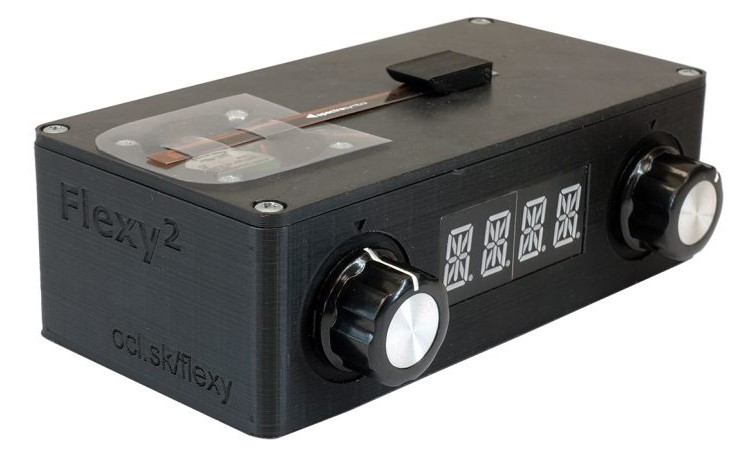
\includegraphics[width=0.5\textwidth]{images/flexy2}
		\caption{Flexy2 device~\cite{flexy2}.}
		\label{fig:flexy2}
	\end{center}
\end{figure}

The model of the system was obtained through experimental identification based on several step responses. The matrices of the nominal state-space system, discretized with sampling time $T_\mathrm{s} = 0.01$\,s are:
\begin{subequations}
	\label{eq:model_A_B} 
	\begin{eqnarray}
		A &=& \begin{bmatrix}
			0.966
		\end{bmatrix}, \quad % \\
		% B &=& \begin{bmatrix}
		B = \begin{bmatrix}
			0.101
		\end{bmatrix}. 
	\end{eqnarray}
\end{subequations}

As the controlled as well as the manipulated variable were set in percentage, their values were constrained from $b_{\min} = v_{\min} = 0\%$ to $b_{\max} = v_{\max} = 100\%$. Considering the steady-state values where the model was linearized, i.e., $ v^\mathrm{s} = 40\%$ and $ b^\mathrm{s} = 68\%$, the constraints were set in both presented control methods as follows: 
\begin{subequations}
	\label{eq:const_u_y} 
	\begin{eqnarray}
	\label{eq:const_u}
	-40\% \le u \le 60\%, \\
	\label{eq:const_y}
	-68\% \le x \le 32\%.
	\end{eqnarray}
\end{subequations}

The rest of the two explicit MPC setups is described in the next sections, according to the specific control approach, as the controllers differ in their structutres and tuning parameters. Both controllers were constructed in MATLAB 2020b programming environment, using toolboxes YALMIP R20210331, MPT 3.2.1, MPTplus,
and solver Gurobi 9.1.1. The explicit MPCs were executed on
CPU AMD Ryzen 7 PRO 4750U, 1.7 GHz with 16 GB RAM.

\subsection{Tube explicit MPC with $\Delta-u$ constraints}
\label{sec:tube_exp}
In this section, the implementation of tube explicit MPC with $\Delta-u$ constraints is described. Let us consider the system model in Eq.~\eqref{eq:model_A_B} and constraints stated in Eq.~\eqref{eq:const_du}. 
As the uncertainties in the model were considered, the additive disturbance was considered in the MPC desing as well and was constrained as:
\begin{eqnarray}
	\label{eq:const_w}
	-1\% \le w \le 1\%.
\end{eqnarray}

Moreover, the change of the input variable was set to validate the control method implemented in the toolbox:
\begin{eqnarray}
	\label{eq:const_du}
	-55\% \le \Delta u \le 55\%.
\end{eqnarray}

By systematic tuning, the penalty matrices of the optimization problem in Eq.~\eqref{eq:tmpc} were set as:
\begin{subequations}
	\label{eq:setup_penalty} 
	\begin{eqnarray}
		\label{eq:setup_Q}
		Q &=& 10, \\
		\label{eq:setup_R}
		R &=& 1.
	\end{eqnarray}
\end{subequations}

The terminal penalty matrix $P$ was set as the LQR penalty, i.e.:
\begin{eqnarray}
	\label{eq:setup_P}
	P = 95.3852.
\end{eqnarray}

Furthermore, the terminal set was constructed as the LQR set and is defined by the following inequality:
\begin{eqnarray}
	\label{eq:setup_terminal_set}
	\begin{bmatrix}
	-1 \\	
	\,\,\,\,\, 1
	\end{bmatrix} x \le 
	\begin{bmatrix}
		31.8694\\	
		21.2463
	\end{bmatrix}
\end{eqnarray}

Last but not least, the prediction horizon $N$ was set to 30 steps. After the construction of the tube explicit model predictive controller, the disturbance rejection control problem was investigated. The control results can be seen in Fig.~\ref{fig:deltaU_y} for the controlled variable, i.e., the flex sensor bend $b$. In Fig.~\ref{fig:deltaU_u}, the corresponding trajectory of manipulated variable is depicted, i.e., the trajectory of fan speed $v$. The aim was to drive the flex sensor bend to the steady state $ b^\mathrm{s} = 68\%$, while rejecting the effect of the two disturbances occuring at times 5\,s and 10\,s. 

\begin{figure}
	\begin{center}
		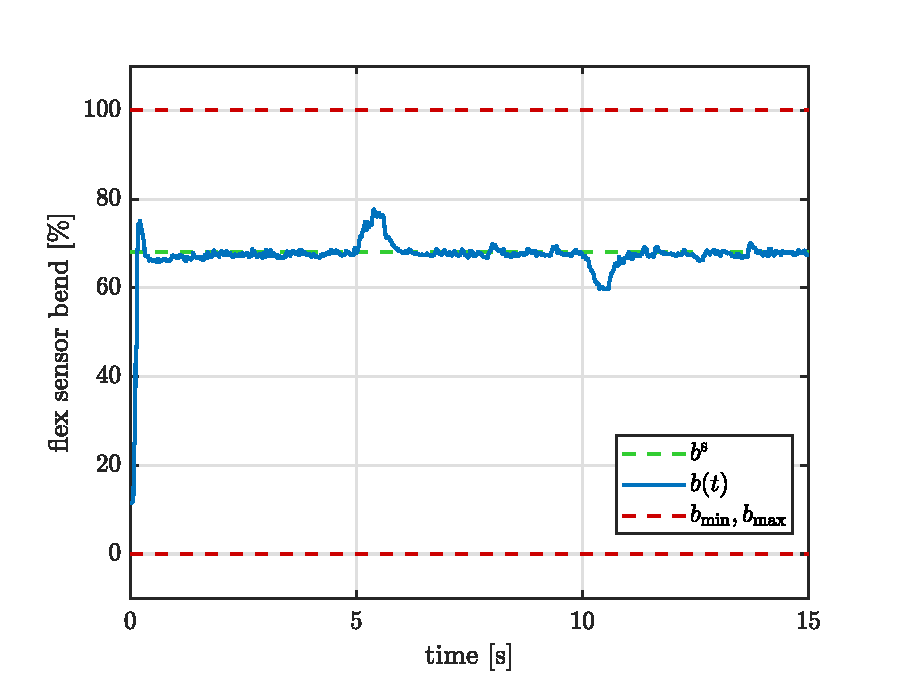
\includegraphics[width=0.5\textwidth]{images/deltaU_b_new.eps}
		\caption{Tube MPC with $\Delta - u$ constraints. Trajectory of controlled variable.}
		\label{fig:deltaU_y}
	\end{center}
\end{figure}

\begin{figure}
	\begin{center}
		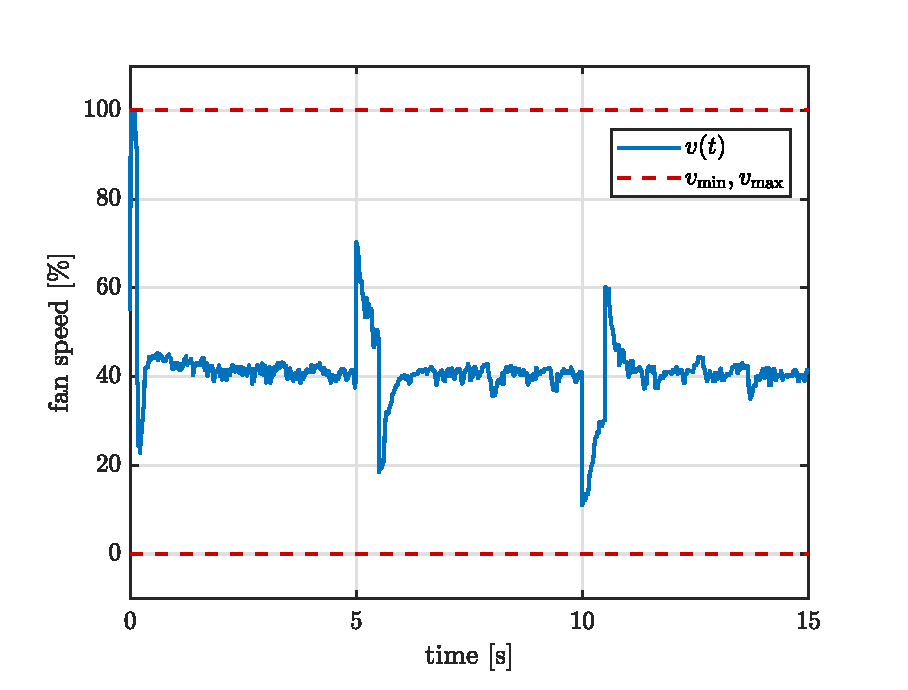
\includegraphics[width=0.5\textwidth]{images/deltaU_v_new.eps}
		\caption{Tube MPC with $\Delta - u$ constraints. Trajectory of manipulated variable.}
		\label{fig:deltaU_u}
	\end{center}
\end{figure}

When observing Fig.~\ref{fig:deltaU_y} and Fig.~\ref{fig:deltaU_u}, it can be seen that the goal of the control was achieved. The effects of both disturbances were rejected, with respect to the constraints on the manipulated and controlled variable. Moreover, the constraints on the change of the manipulated variable were satisfied as well.

\subsection{Polynomial approximation of explicit MPC}
\label{sec:polynomial_exp}
This case study focuses on the second contribution of this work, i.e., the implementation of the explicit MPC approximated with a polynomial. In this approach, the MPC setup in Eq.~(TODO:ref) was considered. Let us consider the system model in Eq.~\eqref{eq:model_A_B} and constraints stated in Eq.~\eqref{eq:const_du}. By systematic tuning, the penalty matrices of the optimization problem in Eq.~(TODO:ref) were set as:
\begin{subequations}
	\label{eq:setup_penalty_pol} 
	\begin{eqnarray}
		\label{eq:setup_Q_pol}
		Q &=& 10, \\
		\label{eq:setup_R_pol}
		R &=& 1.
	\end{eqnarray}
\end{subequations}

The prediction horizon was set as 10 steps long. Based on the aforementioned parameters, the explicit MPC was constructed. Next, the polynomial controller was created based on the optimal one. The degree of the polynomial was determined to 3\textsuperscript{rd} degree. The approximation of the optimal control law can be seen in Fig.~\ref{fig:approx}
 

\begin{figure}
	\begin{center}
		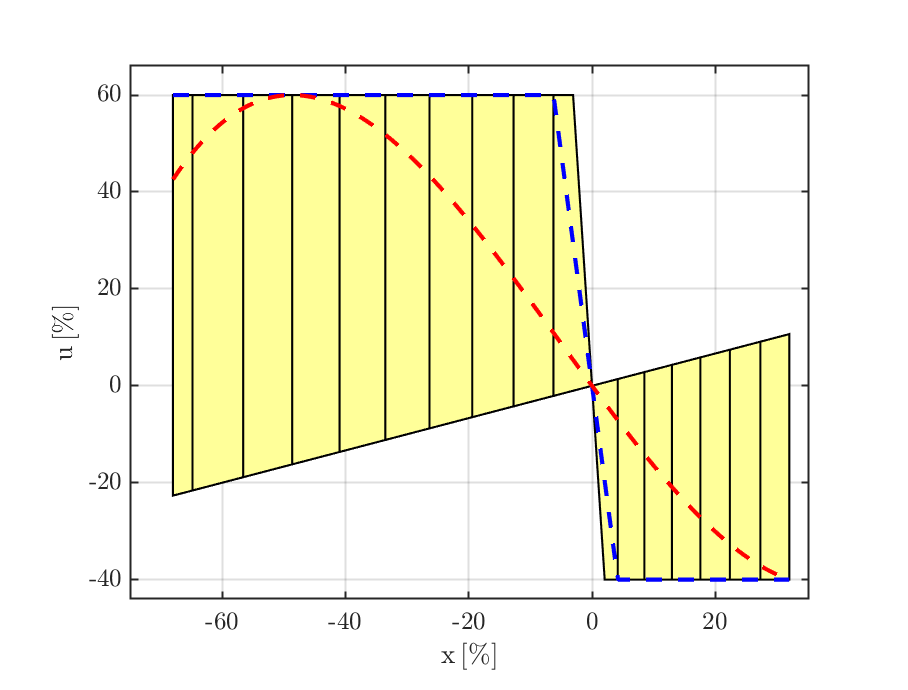
\includegraphics[width=0.5\textwidth]{images/approximation.eps}
		\caption{Approximation of the optimal eMPC. The blue line represents the optimal control law, the yellow area is stability tube, and the red line represents the polynomial approximation of the optimal control law.}
		\label{fig:approx}
	\end{center}
\end{figure}

The comparison of the control results can be seen in Fig.~\ref{fig:poly_y} for the controlled variable and in Fig.~\ref{fig:poly_u} for the manipulated variable. In both graphs, two trajectories are depicted - for the original optimal controller with subscript ,,o'' and its polynomial approximation with subscpript ,,p''. Analogously to the first case study, the aim was to drive the flex sensor bend to the steady state $ b^\mathrm{s} = 68\%$, while rejecting the effect of the two disturbances occuring at times 5\,s and 10\,s.

\begin{figure}
	\begin{center}
		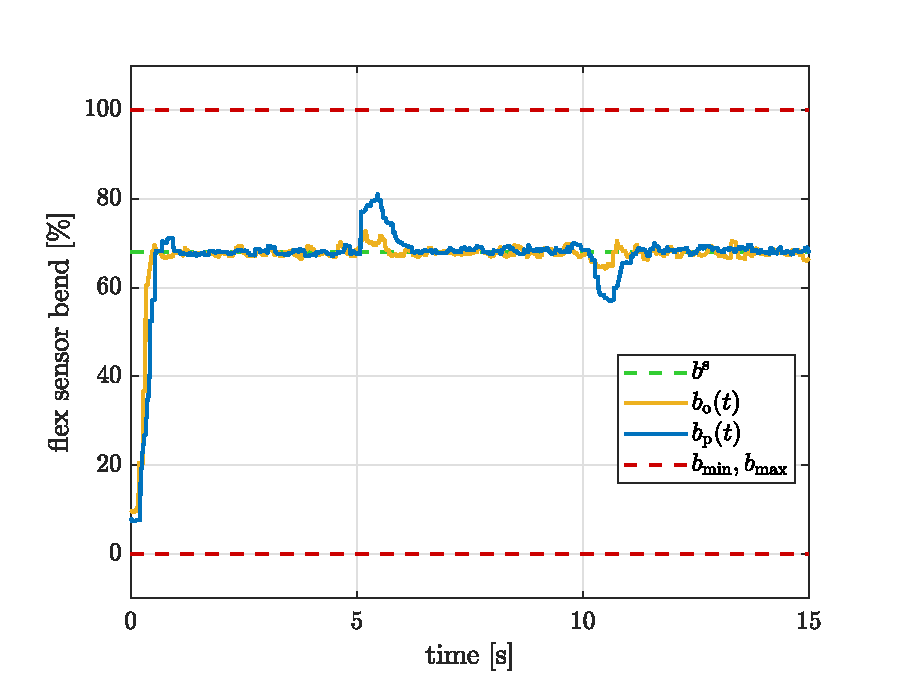
\includegraphics[width=0.5\textwidth]{images/poly_b.eps}
		\caption{Comparison of optimal eMPC and its polynomial approximation. Trajectory of controlled variable.}
		\label{fig:poly_y}
	\end{center}
\end{figure}

\begin{figure}
	\begin{center}
		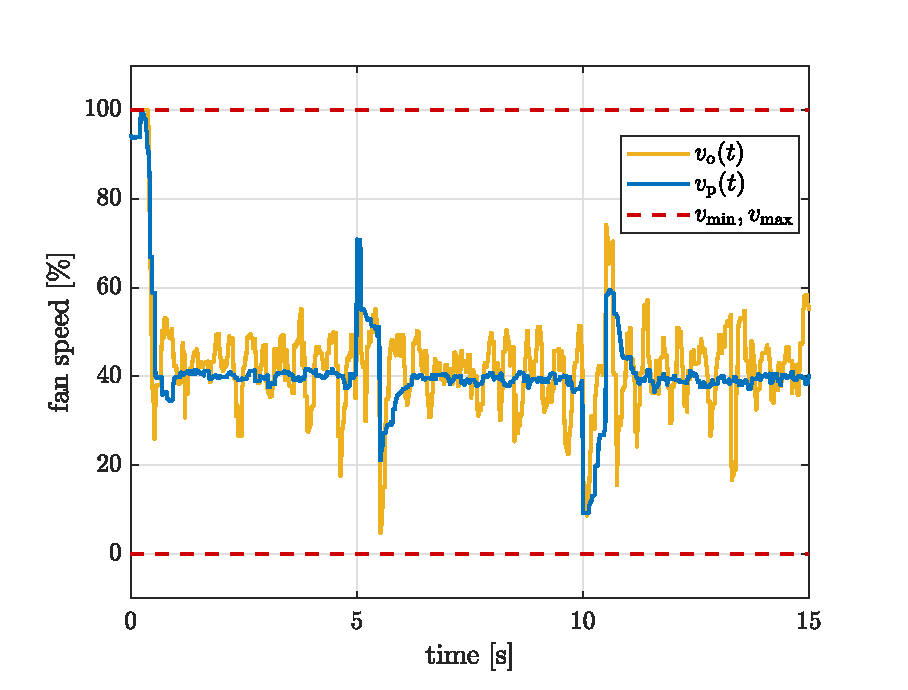
\includegraphics[width=0.5\textwidth]{images/poly_v.eps}
		\caption{Comparison of optimal eMPC and its polynomial approximation. Trajectory of manipulated variable.}
		\label{fig:poly_u}
	\end{center}
\end{figure}

It can be seen in Fig.~\ref{fig:poly_y}, that both disturbances were successfully rejected. Compared to the optimal controller, the approximated one was less oscillating in terms of manipulated variable, see Fig.~\ref{fig:poly_u}. With more cautious control inputs, the effect of the disturbance on the trajectory of controlled variable is more significant. The reason of less oscillating control inputs can be seen in Fig.~\ref{fig:approx}. The original control law is more steep around the origin, while the polynomial approximation is quite moderate. The approximation can be further tuned by setting the polynomial order, which at the end of the day affects the control performance.

%---------------EXAMPLE OF TABLE-----------------
%\begin{table}[h]
%\caption{An Example of a Table}
%\label{table_example}
%\begin{center}
%\begin{tabular}{|c||c|}
%\hline
%One & Two\\
%\hline
%Three & Four\\
%\hline
%\end{tabular}
%\end{center}
%\end{table}
	
 
\section{Conclusions}
\label{sec:conclusions}

[ TOOD: Summarize the main conclusions. ]

The paper presented a detailed tutorial for Tube MPC design using the novel package extension for \texttt{MPT} toolbox. 

\addtolength{\textheight}{-12cm}

\section*{Acknowledgemnts}

[ TODO: Double-check Acks. ]

This research is funded by the European Commission under the grant no. 101079342 (Fostering Opportunities Towards Slovak Excellence in Advanced Control for Smart Industries). The authors gratefully acknowledge the contribution of the Scientific Grant Agency of the Slovak Republic under the grants 1/0545/20, 1/0297/22, and the Slovak Research and Development Agency under the project APVV-20-0261. 



\bibliographystyle{IEEEtran} % use IEEEtran.bst style
% \small
\bibliography{references}


\end{document}
